% Process Model and Planning for SERS
\section{Process Model and Planning}
\begin{itemize}
  

\item \textbf{Process Model Selection}\\
For the Smart Event Reminder System (SERS), the team adopts the \textbf{Agile Scrum} model.

Scrum is selected because the project has a short duration (approximately two weeks), involves evolving requirements, and requires continuous integration between multiple components such as the user interface, backend logic, and asynchronous notification system. Compared to the Waterfall model, Scrum allows the team to quickly adapt to unexpected issues (e.g., scheduling errors or integration problems). Compared to the Incremental model, Scrum provides more structured collaboration through regular meetings and feedback loops.

Therefore, Scrum is the most suitable model for ensuring flexibility, collaboration, and timely delivery.

\item \textbf{Product Backlog}\\
The Product Backlog contains all features required for the system, prioritized based on importance:

\begin{table}[H]
\centering
\caption{Product Backlog}
\begin{tabular}{|l|p{0.55\textwidth}|l|}
\hline
\textbf{ID} & \textbf{Backlog Item} & \textbf{Priority} \\
\hline
PB1 & Create event (title, date, time) & Must \\
\hline
PB2 & Edit event & Must \\
\hline
PB3 & Delete event & Must \\
\hline
PB4 & Schedule reminder & Must \\
\hline
PB5 & Send notification & Should \\
\hline
PB6 & User authentication & Should \\
\hline
PB7 & Share event & Could \\
\hline
\end{tabular}
\end{table}

\item \textbf{Effort Estimation (Planning Poker)}\\
The team uses Planning Poker with Fibonacci scale (0, 1, 2, 3, 5, 8, 13, 21) to estimate effort:

\begin{table}[H]
\centering
\caption{Story Points Estimates}
\begin{tabular}{|p{0.45\textwidth}|c|}
\hline
\textbf{Backlog Item} & \textbf{Story Points} \\
\hline
Database schema & 3 \\
\hline
CRUD API & 8 \\
\hline
Basic UI & 10 \\
\hline
Schedule reminder & 8 \\
\hline
Send notification & 5 \\
\hline
Authentication & 8 \\
\hline
Share event & 3 \\
\hline
\end{tabular}
\end{table}

\item \textbf{Sprint Planning}\\
The project is divided into two sprints (1 week each), ensuring incremental delivery.

Sprint 1: Core System Setup (21 Story Points)
The team commits to the following backlog items:
\begin{itemize}
  \item Initialize database schema (3 points)
  \item Implement CRUD API for events (8 points)
  \item Develop basic UI dashboard (10 points)
\end{itemize}

\noindent\textbf{Total:} 21 story points

This sprint focuses on delivering a functional core system (Minimum Viable Product -- MVP), allowing users to create, view, edit, and delete events.

---

Sprint 2: Advanced Features (Remaining Story Points)
The second sprint focuses on extending system functionality:
\begin{itemize}
  \item Reminder scheduling (8 points)
  \item Notification system (5 points)
  \item User authentication (8 points)
  \item Event sharing (3 points, optional)
\end{itemize}

This sprint enhances the system by adding automation, security, and additional user features.

---

This two-sprint structure ensures that a working system is delivered early (Sprint 1), while advanced capabilities are incrementally added in Sprint 2.

\item \textbf{Team Task Distribution}\\
To support parallel development, tasks are distributed among five team members:
\begin{itemize}
  \item Member A: Backend (CRUD API, database)
  \item Member B: Frontend (UI dashboard)
  \item Member C: Asynchronous system (reminder \& notification)
  \item Member D: Testing and QA
  \item Member E: Documentation and integration
\end{itemize}

\item \textbf{Sprint Day (Simulated 10-Day Cycle)}\\


\begin{table}[H]
\centering
\caption{Sprint Day (Simulated 10-Day Cycle)}
\begin{tabular}{|l|c|p{0.55\textwidth}|}
\hline
\textbf{Day} & \textbf{Remaining Story Points} & \textbf{Progress Narrative} \\
\hline
Day 1 & 21 Points & The sprint begins. All parallel workstreams initiate development on their assigned components. \\
\hline
Day 3 & 18 Points & The database schema architecture is finalized and committed. Points are burned down successfully. \\
\hline
Day 6 & 10 Points & The RESTful API backend logic is completed. The team maintains pace with the ideal burndown trajectory. \\
\hline
Day 8 & 8 Points & A slight plateau occurs. The frontend integration encounters cross-origin resource sharing (CORS) errors, delaying the dashboard completion. \\
\hline
Day 10 & 0 Points & Integration issues are resolved. The dashboard is completed, and all sprint objectives are achieved prior to the sprint review. \\
\hline
\end{tabular}
\end{table}
\begin{figure}[H]
  \centering
  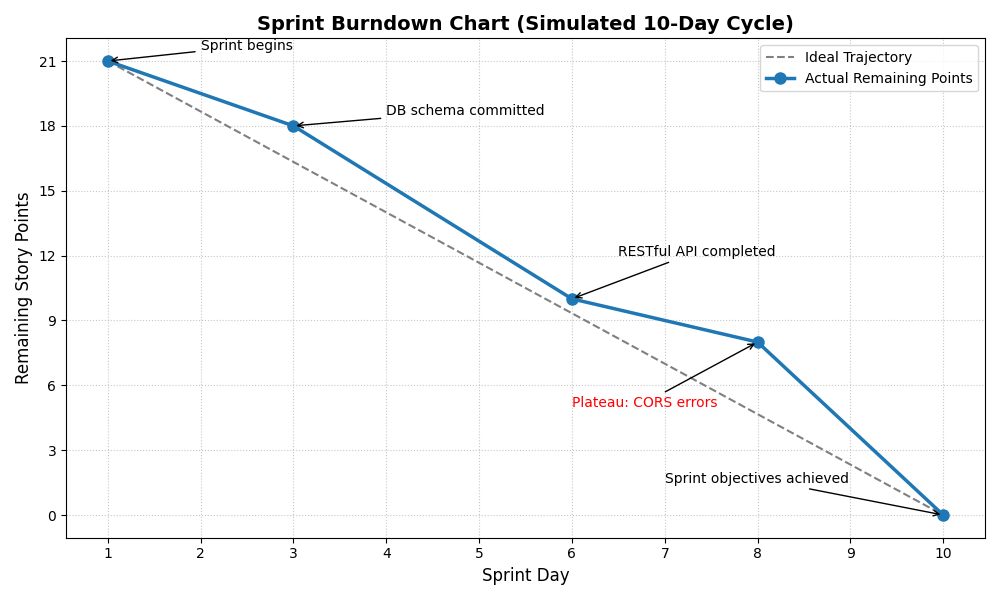
\includegraphics[width=0.8\textwidth]{images/burndown_chart.png}
  \caption{Burndown chart (Simulated 10-Day Cycle)}
  \label{fig:burndown}
\end{figure}

\item \textbf{Summary}\\
Using Scrum enables the team to manage work effectively, adapt to technical challenges, and deliver the system incrementally. The use of backlog prioritization, effort estimation, and sprint planning ensures that the project remains organized and achievable within the given timeframe.
\end{itemize}